%!TEX root =../../course-notes.tex
% ^ leave for LaTeXTools build functionality

\begin{module}{Module G: Geometry of Linear Maps}

\begin{moduleStandards}
  \item \textbf{G1. Determinants}
        Compute the determinant of a square matrix.
  \item \textbf{G2. Eigenvalues}
        Find the eigenvalues of a square matrix, along with their algebraic multiplicities.
  \item \textbf{G3. Eigenvectors}
        Find the eigenspace of a square matrix associated to a given eigenvalue.
   \item \textbf{G4. Geometric multiplicity}
        Compute the geometric multiplicity of an eigenvalue of a square matrix.
\end{moduleStandards}

%!TEX root =../../course-notes.tex
% ^ leave for LaTeXTools build functionality

\begin{readinessAssuranceOutcomes}
\item Calculate the area of a parallelogram.
\item Find the matrix corresponding to a linear transformation of Euclidean spaces \standardList{A1}.
\item Recall and use the definition of a linear transformation \standardList{A2}.
\item Find all roots of quadratic polynomials (including complex ones), and be able to use the rational root theorem to find all rational roots of a higher degree polynomial.
\item Interpret the statement ``$A$ is an invertible matrix'' in many equivalent ways in different contexts.
\end{readinessAssuranceOutcomes}

\begin{readinessAssuranceResources}
\item Finding the area of a parallelogram: \url{https://www.khanacademy.org/math/basic-geo/basic-geo-area-and-perimeter/parallelogram-area/a/area-of-parallelogram}
\item Factoring quadratics: \url{https://www.khanacademy.org/math/algebra2/polynomial-functions/factoring-polynomials-quadratic-forms-alg2/v/factoring-polynomials-1}
\item Finding complex roots of quadratics: \url{https://www.khanacademy.org/math/algebra2/polynomial-functions/quadratic-equations-with-complex-numbers/v/complex-roots-from-the-quadratic-formula}
\item Finding all roots of polynomials: \url{https://www.khanacademy.org/math/algebra2/polynomial-functions/finding-zeros-of-polynomials/v/finding-roots-or-zeros-of-polynomial-1}
\item The Rational Root Theorem:
\url{https://artofproblemsolving.com/wiki/index.php?title=Rational_Root_Theorem}
\end{readinessAssuranceResources}




\begin{readinessAssuranceTest}

%A
\item Find the area of the parallelogram with vertices $(0,0)$, $(4,0)$, $(5,2)$, and $(1,2)$.
\begin{multicols}{2}
\begin{readinessAssuranceTestChoices}
\item $8$ %Correct
\item $10$
\item $12$
\item $14$
\end{readinessAssuranceTestChoices}


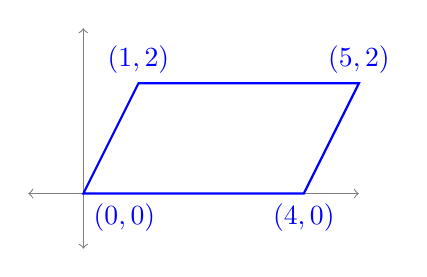
\begin{tikzpicture}[scale=0.7]
\draw[thin,gray,<->] (-1,0)-- (5,0);
\draw[thin,gray,<->] (0,-1)-- (0,3);
\draw[thick,blue] (0,0) node[below right] {$(0,0)$} -- (4,0)node [below] {$(4,0)$} -- (5,2) node[above] {$(5,2)$} -- (1,2) node[above]{$(1,2)$} -- cycle;
\end{tikzpicture}
\end{multicols}

%A
\item Find the area of the parallelogram with vertices $(0,0)$, $(12,5)$, $(12,8)$, and $(0,3)$.
\begin{multicols}{2}
\begin{readinessAssuranceTestChoices}
\item $36$ %Correct
\item $54$
\item $72$
\item $96$
\end{readinessAssuranceTestChoices}


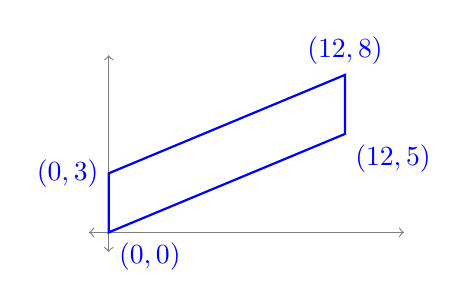
\begin{tikzpicture}[scale=0.25]
\draw[thin,gray,<->] (-1,0)-- (15,0);
\draw[thin,gray,<->] (0,-1)-- (0,9);
\draw[thick,blue] (0,0) node[below right] {$(0,0)$} -- (12,5)node [below right] {$(12,5)$} -- (12,8) node[above] {$(12,8)$} -- (0,3) node[left]{$(0,3)$} -- cycle;
\end{tikzpicture}
\end{multicols}

%D
\item The parallelogram ABCD has area $6$.  If AE is $50\%$ longer than AB, what is the area of the parallelogram AEFD?
\begin{multicols}{2}
\begin{readinessAssuranceTestChoices}
\item $18$
\item $15$
\item $12$
\item $9$  %Correct
\end{readinessAssuranceTestChoices}

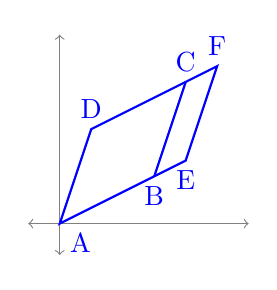
\begin{tikzpicture}[scale=0.4]
\draw[thin,gray,<->] (-1,0)-- (6,0);
\draw[thin,gray,<->] (0,-1)-- (0,6);
\draw[thick,blue] (0,0) node[below right] {A} --(4,2) node[below] {E} -- (5,5) node[above]{F} -- (1,3)node[above] {D} -- cycle;
\draw[thick,blue] (3,1.5) node[below] {B} -- (4,4.5) node [above] {C};
\end{tikzpicture}
\end{multicols}

%C
\item The parallelogram ABCD has area $6$.  If AD is twice as long as AF, what is the area of the parallelogram ABEF?
\begin{multicols}{2}
\begin{readinessAssuranceTestChoices}
\item $1$
\item $2$
\item $3$ %Correct
\item $4$
\end{readinessAssuranceTestChoices}

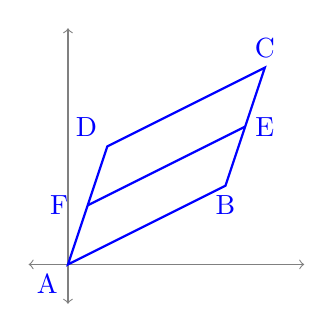
\begin{tikzpicture}[scale=0.5]
\draw[thin,gray,<->] (-1,0)-- (6,0);
\draw[thin,gray,<->] (0,-1)-- (0,6);
\draw[thick,blue] (0,0) node[below left] {A} --(4,2) node[below] {B} -- (5,5) node[above]{C} -- (1,3)node[above left] {D} -- cycle;
\draw[thick,blue] (0.5,1.5) node[left] {F\ \ } -- (4.5,3.5) node [right] {E};
\end{tikzpicture}
\end{multicols}

%A
\item Let $T: \IR^2 \rightarrow \IR$ be a linear transformation.  Which of the following is equal to $2T\left(\begin{bmatrix} a+b \\ a+b \end{bmatrix}\right)$?
\begin{multicols}{2}
\begin{readinessAssuranceTestChoices}
\item $T\left(\begin{bmatrix} a \\ a \end{bmatrix}\right)+T\left(\begin{bmatrix}a \\ b \end{bmatrix} \right)+T\left(\begin{bmatrix}b \\ a \end{bmatrix}\right)+T\left(\begin{bmatrix}b \\ b \end{bmatrix} \right)$ %Correct
\item $T\left(\begin{bmatrix}a \\ b \end{bmatrix} \right)+T\left(\begin{bmatrix}b \\ a \end{bmatrix} \right)$
\item $T\left(\begin{bmatrix}a \\ b \end{bmatrix} \right)$
\item $2T\left(\begin{bmatrix}a \\ b \end{bmatrix} \right)$
\end{readinessAssuranceTestChoices}
\end{multicols}

%D
\item Let $T: \IR^n \rightarrow \IR^n$ be a linear transformation with standard matrix $A$.  Which of the following is equivalent to the statement ``$A$ is an invertible matrix''?
\begin{readinessAssuranceTestChoices}
\item $A$ is a square matrix
\item The matrix equation $AX=B$ has no solution for some $n\times 1$
      matrix $B$.
\item $\RREF(A)$ has a column without a pivot
\item $T$ is both injective and surjective %Correct
\end{readinessAssuranceTestChoices}

%B
\item What is the matrix corresponding to the linear transformation $T: \IR^3 \rightarrow \IR^3$ given by $$T\left( \begin{bmatrix} x \\ y \\ z \end{bmatrix}\right) = \begin{bmatrix} 3x+2y-z \\ y+z \\x+7z \end{bmatrix}?$$
\begin{multicols}{4}
\begin{readinessAssuranceTestChoices}
\item $\begin{bmatrix} 3 & 0 & 1 \\ 2 & 1 & 0 \\ -1 & 1 & 7 \end{bmatrix}$
\item $\begin{bmatrix} 3 & 2 & -1 \\ 0 & 1 & 1 \\ 1 & 0 & 7  \end{bmatrix}$ %Correct
\item $\begin{bmatrix} 3 & 2 & -1 \\ 1 & 1 & 0 \\ 1 & 7 & 0 \end{bmatrix}$
\item $\begin{bmatrix}  3 & 1 & 1 \\ 2 & 1 & 7 \\ -1 & 0 & 0 \end{bmatrix}$
\end{readinessAssuranceTestChoices}
\end{multicols}

%B
\item How many distinct real roots does the polynomial $x^4+3x^3+x^2-3x-2$ have?
(Hint: all the roots are rational.)
\begin{multicols}{4}
\begin{readinessAssuranceTestChoices}
\item $4$
\item $3$ %Correct
\item $2$
\item $1$
\end{readinessAssuranceTestChoices}
\end{multicols}


%A
\item Which of the following is a root of the polynomial $x^2-4x+13$?
\begin{multicols}{4}
\begin{readinessAssuranceTestChoices}
\item $2-3i$ %Correct
\item $3+4i$
\item $4-5i$
\item $5+6i$
\end{readinessAssuranceTestChoices}
\end{multicols}

%A
\item Which of the following conditions imply that the quadratic polynomial $ax^2+bx+c$ has no real roots?
\begin{multicols}{2}
\begin{readinessAssuranceTestChoices}
\item $b^2-4ac<0$ %Correct
\item $a^2+4bc<0$
\item $ac-4b^2<0$
\item $ab+4c^2<0$
\end{readinessAssuranceTestChoices}
\end{multicols}

\end{readinessAssuranceTest}

%!TEX root =../../course-notes.tex
% ^ leave for LaTeXTools build functionality

\begin{applicationActivities}{1}{25}

\begin{activity}{5}
Consider the linear transformation $A : \IR^2 \rightarrow \IR^2$ given by the matrix $A = \begin{bmatrix} 2 & 0 \\ 0 & 3 \end{bmatrix}$

\begin{center}
\begin{tikzpicture}
\draw[thin,gray,<->] (-4,0)-- (4,0);
\draw[thin,gray,<->] (0,-4)-- (0,4);
\draw[thick,blue,->] (0,0) -- node[below] {$A \vec{e}_1$}++ (2,0);
\draw[thick,blue,->] (0,0) -- node[left] {$A \vec{e}_2$}++(0,3);
\draw[blue,dashed] (2,0) -- (2,3) -- (0,3);
\end{tikzpicture}
\end{center}

We can summarize the transformation of the unit square into this rectangle by measuring the following:

\begin{enumerate}[(a)]
\item How did the area change?
\item How was th $x$-axis stretched?
\item How was the $y$-axis stretched?
\end{enumerate}

\end{activity}


\begin{activity}{15}
Consider the following linear transformations  $A_i: \IR^2 \rightarrow \IR^2$.
\begin{itemize}
\item $A_2 = \begin{bmatrix} 2 & 3 \\ 0 & 1 \end{bmatrix}$
\item $A_3 = \begin{bmatrix} 1 & -1 \\ 1 & 1 \end{bmatrix}$
\item $A_4 = \begin{bmatrix} 0 & 1 \\ 1 & 0 \end{bmatrix}$
\item $A_5 = \begin{bmatrix} 1 & 1 \\ 0 & 0 \end{bmatrix}$
\end{itemize}

For each linear transformation, do the following:
\begin{enumerate}[(a)]
\item Draw a graph showing the image of the unit square.
\item Compute how much the area was stretched out.
\item Determine which axes (or lines) were preserved; how were they stretched out?
\end{enumerate}
\end{activity}

\begin{activity}{10}
Our goal is to define a function $\det:M_n \rightarrow \IR$ that takes a square matrix (linear transformation $\IR^n \rightarrow \IR^n$) and returns its area stretching factor.  This function is called the \term{determinant}.

What properties should this function have?

\begin{minipage}{0.8\textwidth}
Match the four pictures to the following four expressions

\begin{align*}
\det(\vec{e}_1,\vec{e}_2) &&
\det(\vec{v},\vec{v}) &&
\det(c\vec{v},\vec{w})  &&
\det(\vec{u}+\vec{v},\vec{w})
\end{align*}


\begin{multicols}{2}
\begin{center}
\begin{tikzpicture}[scale=1.5]
\draw[thin,gray,<->] (-1,0)-- (3,0);
\draw[thin,gray,<->] (0,-1)-- (0,3);
\draw[thick,blue,->] (0,0) -- node[below] {$\vec{e}_1$} (1,0);
\draw[thick,blue,->] (0,0) -- node[left] {$\vec{e}_2$} (0,1);
\draw[thick,blue,->] (1,0) -- (1,1);
\draw[thick,blue,->] (0,1) -- (1,1);
\end{tikzpicture}
\end{center}

\begin{center}
\begin{tikzpicture}[scale=1.2]
\draw[thin,gray,<->] (-1,0)-- (4,0);
\draw[thin,gray,<->] (0,-1)-- (0,4);
\draw[thick,blue,->] (0,0) -- node[below] {$\vec{v}$} (3,2);
\end{tikzpicture}
\end{center}


\begin{center}
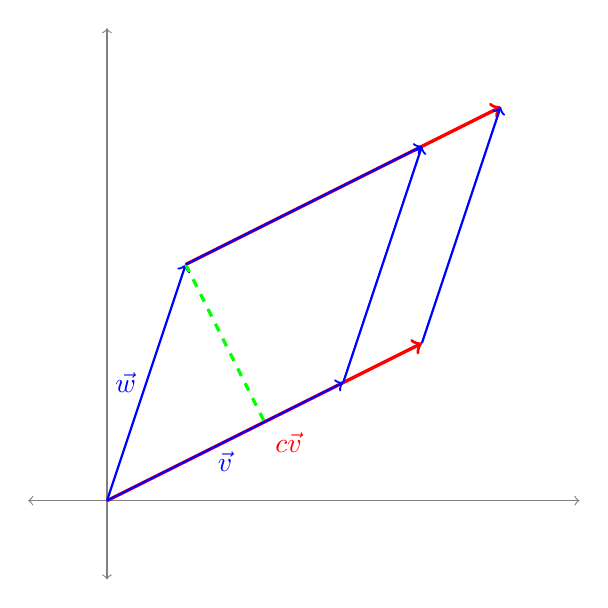
\begin{tikzpicture}
\draw[thin,gray,<->] (-1,0)-- (6,0);
\draw[thin,gray,<->] (0,-1)-- (0,6);
\draw[very thick,red,->] (0,0) -- node[below right] {$c\vec{v}$}  (4,2);
\draw[very thick,red,->] (1,3) -- (5,5);
\draw[thick,blue,->] (0,0) -- node[below] {$\vec{v}$} (3,1.5);
\draw[thick,blue,->] (0,0) -- node[left] {$\vec{w}$} (1,3);
\draw[green,very thick,dashed] (1,3) -- (2,1);
\draw[thick,blue,->] (3,1.5) -- (4,4.5);
\draw[thick,blue,->] (1,3) -- (4,4.5);


\draw[thick,blue,->] (4,2) -- (5,5);
\end{tikzpicture}
\end{center}

\begin{center}
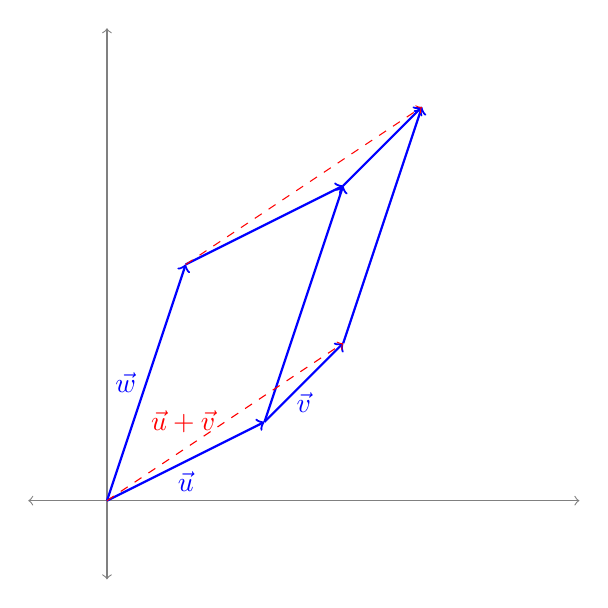
\begin{tikzpicture}
\draw[thin,gray,<->] (-1,0)-- (6,0);
\draw[thin,gray,<->] (0,-1)-- (0,6);
\draw[thick,blue,->] (0,0) -- node[below] {$\vec{u}$} (2,1);
\draw[thick,blue,->] (0,0) -- node[left] {$\vec{w}$} (1,3);
\draw[thick,blue,->] (2,1) -- node [below] {$\vec{v}$}(3,2);
\draw[thick,blue,->] (2,1) -- (3,4);
\draw[thick,blue,->] (3,2) -- (4,5);
\draw[thick,blue,->] (1,3) -- (3,4);
\draw[thick,blue,->] (3,4) -- (4,5);
\draw[dashed,red,->] (0,0) -- node[above,left] {$\vec{u}+\vec{v}$} (3,2);
\draw[dashed,red,->] (1,3) -- (4,5);
\end{tikzpicture}
\end{center}

\end{multicols}
\end{minipage}

\end{activity}

\begin{activity}{10}
What can you conclude about each of the following?
\begin{enumerate}
\item $\det(\vec{e}_1,\vec{e}_2)$
\item $\det(\vec{v},\vec{v})$
\item $\det(c\vec{v},\vec{w})$
\item $\det(\vec{u}+\vec{v},\vec{w})$
\end{enumerate}
\end{activity}


\begin{definition}
To summarize, we have 3 properties (stated here over $\IR^n$)
\begin{enumerate}
\item [P1:] $\det(\vec{e}_1,\vec{e}_2,\ldots,\vec{e}_n)=1$
\item [P2:] If $\vec{v}_i = \vec{v}_j$ for some $i \neq j$, then $\det(\vec{v}_1,\vec{v}_2,\ldots,\vec{v}_n)=0$.
\item[P3:] The determinant is linear in each column.
\end{enumerate}

These three properties uniquely define the \term{determinant}, as we shall see.
\end{definition}

\begin{observation}
Note that if $\vec{v},\vec{w} \in \IR^2$ and $A=\begin{bmatrix} \vec{v} & \vec{w}\end{bmatrix}$ we will write either $\det(A)$ or $\det(\vec{v},\vec{w})$ as is convenient.
\end{observation}

\begin{activity}{5}
How are $\det (\vec{v},\vec{w})$ and $\det(\vec{w},\vec{v})$ related?
\begin{enumerate}[(a)]
\item $\det(\vec{v},\vec{w}) = \det(\vec{w},\vec{v})$
\item $\det(\vec{v},\vec{w}) = -\det(\vec{w},\vec{v})$
\item They are unrelated
\item They are related, but not by either (a) or (b).
\end{enumerate}
\end{activity}


\begin{observation}
Note that this implies that the determinant is actually a \textit{signed} area (volume)!
\end{observation}

\begin{activity}{5}
How are $\det (\vec{v}+\vec{w},\vec{w})$ and $\det(\vec{v},\vec{w})$ related?
\begin{enumerate}[(a)]
\item $\det(\vec{v}+\vec{w},\vec{w}) = \det(\vec{v},\vec{w})$
\item $\det(\vec{v}+\vec{w},\vec{w}) = -\det(\vec{v},\vec{w})$
\item They are unrelated
\item They are related, but not by either (a) or (b).
\end{enumerate}
\end{activity}

\begin{observation}
  Note that we now understand the effect of any column operation on the determinant.
\end{observation}


\end{applicationActivities}
 % includes Day 2
%!TEX root =../../course-notes.tex
% ^ leave for LaTeXTools build functionality

\begin{applicationActivities}{3}{27}

\begin{activity}{5}
  Suppose the matrix \(M\) is invertable, so there exists \(M^{-1}\)
  with \(MM^{-1}=I\). It follows that \(\det(M)\det(M^{-1})=\det(I)\).

  What is the only number that \(\det(M)\) cannot equal?
  \begin{multicols}{4}
  \begin{enumerate}[(a)]
  \item \(-1\)
  \item \(0\)
  \item \(1\)
  \item \(\frac{1}{\det(M^{-1})}\)
  \end{enumerate}
  \end{multicols}
\end{activity}

\begin{fact}
  Since \(\det(M^{-1})=\frac{1}{\det(M)}\) for every invertable matrix \(M\),
  a square matrix \(M\) is invertable if and only if \(\det(M)\not=0\).
\end{fact}

\begin{observation}
Consider the linear transformation $A : \IR^2 \rightarrow \IR^2$ given by the matrix $A = \begin{bmatrix} 2 & 2 \\ 0 & 3 \end{bmatrix}$

\begin{center}
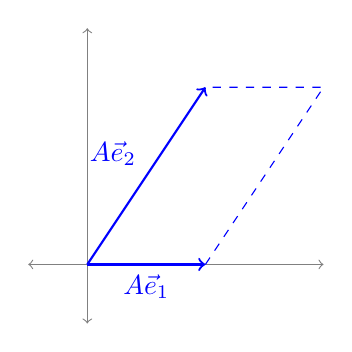
\begin{tikzpicture}[scale=0.75]
\draw[thin,gray,<->] (-1,0)-- (4,0);
\draw[thin,gray,<->] (0,-1)-- (0,4);
\draw[thick,blue,->] (0,0) -- node[below] {$A \vec{e}_1$}++ (2,0);
\draw[thick,blue,->] (0,0) -- node[above left] {$A \vec{e}_2$}++(2,3);
\draw[blue,dashed] (2,0) -- (4,3) -- (2,3);
\end{tikzpicture}
\end{center}
It is easy to see geometrically that  $$ A\begin{bmatrix}1 \\ 0 \end{bmatrix} = \begin{bmatrix}2 \\ 0 \end{bmatrix}= 2 \begin{bmatrix}1 \\ 0 \end{bmatrix}$$

It is less obvious (but easily verified by computation) that
$$A\begin{bmatrix} 2 \\ 1 \end{bmatrix} = \begin{bmatrix} 6 \\ 3 \end{bmatrix} = 3\begin{bmatrix} 2 \\ 1 \end{bmatrix}$$
\end{observation}

\begin{definition}Let $A \in \IR^{n \times n}$.
An \term{eigenvector} is a vector $\vec{x} \in \IR^n$ such that $A\vec{x}$ is parallel to $\vec{x}$.

In other words, $A\vec{x}=\lambda \vec{x}$ for some scalar $\lambda$.
We call this \(\lambda\) an \term{eigenvalue} of \(A\).
\end{definition}

\begin{observation}
Since \(\lambda\vec x=\lambda (I\vec x)\), we can find the eigenvalues and
eigenvectors satisfying $A\vec{x}=\lambda \vec{x}$ by inspecting
$(A-\lambda I)\vec{x} = \vec0$.
\begin{itemize}
\item Since we already know that $(A-\lambda I)\vec0 = \vec0$
for any value of \(\lambda\),
we are more interested in finding values of $\lambda$ such that
$A-\lambda I$ has a nontrivial kernel.
\item Thus \(\RREF(A-\lambda I)\) must have a non-pivot column, and therefore
\(A-\lambda I\) cannot be invertable.
\item
Since \(A-\lambda I\) cannot be invertable, our eigenvalues must satisfy
\(\det(A-\lambda I)=0\).
\end{itemize}
\end{observation}

\begin{definition}
Computing \(\det(A-\lambda I)\) results in the
\term{characteristic polynomial} of \(A\).

For example, when
\(A=\begin{bmatrix}1 & 2 \\ 3 & 4\end{bmatrix}\), we have

\[
  A-\lambda I=
  \begin{bmatrix}1 & 2 \\ 3 & 4\end{bmatrix}-
  \begin{bmatrix}\lambda & 0 \\ 0 & \lambda\end{bmatrix}=
  \begin{bmatrix}1-\lambda & 2 \\ 3 & 4-\lambda\end{bmatrix}
\]

Thus the characteristic polynomial of \(A\) is

\[
  \det\begin{bmatrix}1-\lambda & 2 \\ 3 & 4-\lambda\end{bmatrix}
=
  (1-\lambda)(4-\lambda)-6
=
  \lambda^2-5\lambda-2
\]
% Computing $\det(A-\lambda I)$ is called the \term{characteristic polynomial} of $A$.  It is a polynomial in the variable $\lambda$.
% \item Once an eigenvalue is found, the eigenvectors form a subspace called the \term{eigenspace}, which is simply the kernel of $A-\lambda I$.  Each eigenvalue will have an associated eigenspace.
\end{definition}

\begin{activity}{15}
  Complete the following computation of the characteristic polynomial
  \(A-\lambda I\) for
  $A=\begin{bmatrix} 6 & -2 & 1 \\ 17 & -5 & 5 \\ -4 & 2 & 1 \end{bmatrix}$.

  \scalebox{.8}{\parbox{1.2\linewidth}{
  \begin{align*}
    \begin{bmatrix} 6-\lambda & -2 & 1 \\ 17 & -5-\lambda & 5 \\ -4 & 2 & 1-\lambda \end{bmatrix}
  &=
    (6-\lambda)\det \begin{bmatrix}
      \unknown & \unknown & \unknown \\
      0 & 1 & -1 \\
      1 & 2 & 0
    \end{bmatrix}
    -2\det \begin{bmatrix}
      \unknown & \unknown & \unknown \\
      0 & 1 & -1 \\
      1 & 2 & 0
    \end{bmatrix}
    +\det \begin{bmatrix}
      \unknown & \unknown & \unknown \\
      0 & 1 & -1 \\
      1 & 2 & 0
    \end{bmatrix}
  \\ &=
    (6-\lambda)\det \begin{bmatrix}
      1 & 0 & 0 \\
      \unknown & \unknown & \unknown \\
      \unknown & \unknown & \unknown \\
    \end{bmatrix}
    +2\det \begin{bmatrix}
      1 & 0 & 0 \\
      \unknown & \unknown & \unknown \\
      \unknown & \unknown & \unknown \\
    \end{bmatrix}
    -\det \begin{bmatrix}
      1 & 0 & 0 \\
      \unknown & \unknown & \unknown \\
      \unknown & \unknown & \unknown \\
    \end{bmatrix}
  \\ &=
    (6-\lambda)\det \begin{bmatrix}
      \unknown & \unknown \\
      \unknown & \unknown \\
    \end{bmatrix}
    +2\det \begin{bmatrix}
      \unknown & \unknown \\
      \unknown & \unknown \\
    \end{bmatrix}
    -\det \begin{bmatrix}
      \unknown & \unknown \\
      \unknown & \unknown \\
    \end{bmatrix}
  \\ &=
    (6-\lambda)((-5-\lambda)(1-\lambda)-10)
    +2(17(1-\lambda)+20)
    -(-4(-5-\lambda)-34)
  \end{align*}}}
\end{activity}

\begin{activity}{15}
Let $A = \begin{bmatrix} 2 & 2 \\ 0 & 3 \end{bmatrix}$.
\begin{subactivity}
Compute $\det \begin{bmatrix} 2-\lambda & 2 \\ 0 & 3-\lambda \end{bmatrix}$ to determine the characteristic polynomial of $A$.
\end{subactivity}
\begin{subactivity}
Find the roots of the characteristic polynomial
to determine the eigenvalues of $A$.
\end{subactivity}
\begin{subactivity}
Compute the kernel of the transformation given by
\[
  A-2I
    =
  \begin{bmatrix} 2-2 & 2 \\ 0 & 3-2 \end{bmatrix}
\] to determine all the eigenvectors associated to the eigenvalue $2$.
\end{subactivity}
\begin{subactivity}
Compute the kernel of the transformation given by $A-3I$ to determine all the eigenvectors associated to the eigenvalue $3$.
\end{subactivity}
\end{activity}

\begin{definition}
  The kernel of the transformation given by \(A-\lambda I\) contains
  all the eigenvectors associated with \(\lambda\). Since kernel is a subspace
  of \(\IR^n\), we call this kernel the \term{eigenspace} associated with the
  eigenvalue \(\lambda\).
\end{definition}


\begin{activity}{15}
  Find all the eigenvalues and associated eigenspaces for the matrix $A=\begin{bmatrix} 3 & -2 & 1 \\  0 & 2 & 8 \\ 0 & 2 & 2 \end{bmatrix}$.

\begin{subactivity}
 Compute $\det (A-\lambda I)$ to determine the characteristic polynomial of $A$.
\end{subactivity}
\begin{subactivity}
Find the roots of the characteristic polynomial
\((3-\lambda)(\lambda^2-4\lambda-12)\)
to determine the eigenvalues of $A$.
\end{subactivity}
\begin{subactivity}
Compute the kernels of $A-\lambda I$ for each eigenvalue
$\lambda\in\{-2,3,6\}$ to determine the respective eigenspaces.
\end{subactivity}
\end{activity}

\end{applicationActivities}

%!TEX root =../../course-notes.tex
% ^ leave for LaTeXTools build functionality

\begin{applicationActivities}{4}{28}
\begin{observation}
Recall from last class:
\begin{itemize}
\item To find eigenvalues the eigenvalues of a matrix $A$, we need to find values of $\lambda$ such that $A-\lambda I$ has a nontrivial kernel; equivalently, $A-\lambda I$ is not invertible, which is equivalent to $\det(A-\lambda I)=0$.  
\item $\det(A-\lambda I)$ is called the \term{characteristic polynomial} of $A$.  It is a polynomial in the variable $\lambda$.
\item Once an eigenvalue is found, the eigenvectors form a subspace called the \term{eigenspace}, which is simply the kernel of $A-\lambda I$.  Each eigenvalue will have an associated eigenspace.
\end{itemize}
\end{observation}

\begin{activity}{5}
  If $A$ is a $4 \times 4$ matrix, what is the largest number of eigenvalues $A$ can have?
  \begin{enumerate}[(a)]
  \item $3$
  \item $4$
  \item $5$
  \item $6$
  \item It can have infinitely many
  \end{enumerate}
\end{activity}

\begin{activity}{10}
  $2$ is an eigenvalue of each of the matrices $A=\begin{bmatrix} 1 & -2 & 1 \\ -1 & 0 & 1 \\ -1 & -2 & 3\end{bmatrix}$ and $B=\begin{bmatrix} -3 & -9 & 5 \\ -2 & -2 & 2 \\ -7 & -13 & 9 \end{bmatrix}$.

  Compute the eigenspace associated to $2$ for both $A$ and $B$.
\end{activity}

\begin{definition}

\begin{itemize}
\item The \term{algebraic multiplicity} of an eigenvalue is its multiplicity as a root of the characteristic polynomial.
\item The \term{geometric multiplicity} of an eigenvalue is the dimension of the eigenspace.
\end{itemize}

\end{definition}

\begin{activity}{5} How are the algebraic and geometric multiplicities related?
\begin{enumerate}[(a)]
\item The algebraic multiplicity is always at least as big as than the geometric multiplicity.
\item The geometric multiplicity is always at least as big as the algebraic multiplicity.
\item Sometimes the algebraic multiplicity is larger and sometimes the geometric multiplicity is larger.
\end{enumerate}
\end{activity}

\begin{activity}{20}
   Find all of the eigenvalues, along with both their algebraic and geometric multiplicities, for the matrix $\begin{bmatrix} -3 & 1 & 2 & 1 \\ -9 & 5 & -2 & -1 \\ 31 & -17 & 6 & 3 \\ -69 & 39 & -18 & -9 \end{bmatrix}$.  Use technology to help you!
\end{activity}



\begin{activity}{10}
Let  $A=\begin{bmatrix}0 & -1 \\ 1 & 0 \end{bmatrix}$.
\begin{subactivity}
  Find the eigenvalues of $A$
  \end{subactivity}
  \begin{subactivity}
   Describe what this linear transformation is doing geometrically; draw a picture.
   \end{subactivity}
\end{activity}



\end{applicationActivities}


\end{module}